% =====================================================================
%  Chapter 6 — The Premium You Are Trying to Capture
% =====================================================================

\chapter{The Premium You Are Trying to Capture}\idx{Premium}
\label{ch:premium}

Before one can ask whether a machine has found an edge, one has to say what
the edge would be an edge \emph{over}. This chapter fixes the target: the
risk premium\idx{Risk premium} available to a long-horizon equity investor, measured on the
book's own data, with the arithmetic carried out here rather than quoted.

\section{What the premium is, precisely}

A premium is not a number of percent. It is a difference between two
quantities that are both random, and the definition has to name the
benchmark, the horizon, the currency and the risk adjustment, or it is
useless.

The book's definition: the risk premium is the excess of the geometric mean
return of a risky asset over the geometric mean return of a riskless asset,
over a stated horizon, net of the costs of transacting and of the taxes on
the returns.

Geometric, because money is compounded and the arithmetic mean is not what
an investor receives. Net, because the difference between a gross and a net
premium is the difference between a strategy that exists and one that does
not. Horizon-stated, because Chapter 8 shows that the horizon changes the
premium by an amount comparable to the premium itself.

\section{What the index did, on this book's own data}

The book's data pipeline pulls daily price and dividend\idx{Dividend} series for every
fund in the universe from a single source, caches them with checksums, and
reconstructs monthly total returns from the price and dividend components
rather than from an adjusted close. Chapter 12 and Appendix A give the
provenance; the point here is only that the numbers are computed here.

The headline series is the S\&P 500 tracker, which has a continuous record
from 1993 in this dataset and is the book's benchmark throughout.

\begin{figure}[!htbp]
\centering
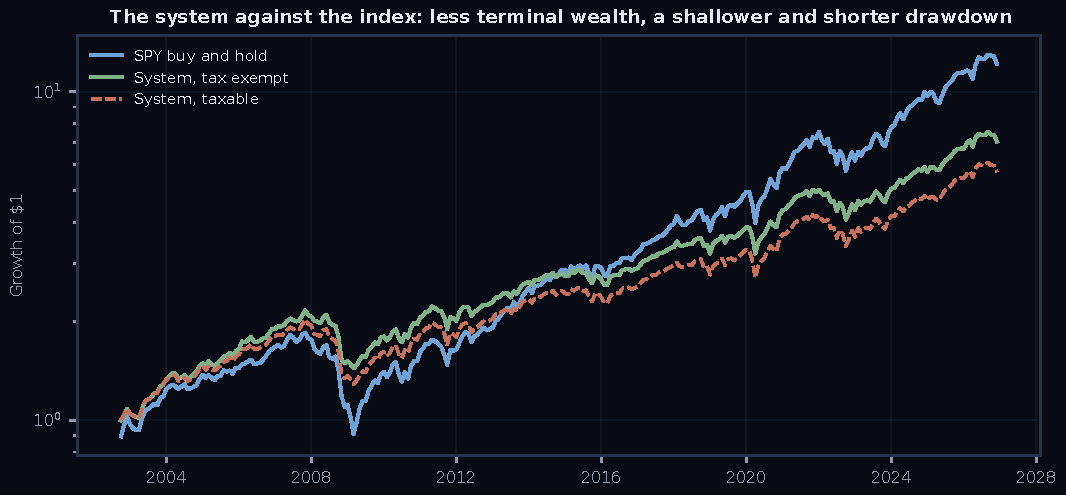
\includegraphics[width=\textwidth]{../figures/fig_wealth.pdf}
\caption{The benchmark and the system, compounded over the record. Both
curves are net of the spread costs charged on every trade the system makes;
the benchmark is gross of nothing because it makes none. The comparison is
made in Part VI.}
\label{fig:wealth}
\end{figure}

Over the full monthly panel, 407 months from January 1993 to November 2026,
the benchmark's total-return compound annual growth rate is
\numSpyFullCAGR{}. Over the system's own record, which begins later
because the model needs a warm-up, the same benchmark returns
\numSpyCAGR{}.

Those two numbers bracket the difficulty of the problem. A CAGR in the high
single digits, sustained over a quarter of a century, is an excellent
outcome; and the strategy that reliably produces it is to do nothing and
own the index. Everything in this book is measured against that.

\section{The components of the premium, and the arithmetic of diversification}

The premium is not a single number either. It is made of parts that behave
differently, and a portfolio that captures one part need not capture
another.

The book works with four sleeves, and each corresponds to a distinct source
of expected excess return.

\textbf{Equity risk.} The premium for bearing the risk of the business of
the economy, over the whole horizon. Historically large and slow-moving.

\textbf{Geographic diversification.} A premium that is not the same premium.
Country-specific returns are strongly negatively correlated with the world
in some periods and not in others, and the academic case for holding a
non-US allocation rests on the currency and fiscal correlation structure
rather than on a separate source of return. The book's stated policy holds
a non-US sleeve for that reason and not for a return premium.

\textbf{Bond risk.} Duration and credit. The premium is different in kind:
it is largely compensation for inflation risk, and it behaves badly in
exactly the regime --- rising real rates --- in which equities\idx{Equities} also behave
badly, which limits the diversification benefit.

\textbf{Real assets.} Commodities and real estate. A premium with a
distinct and rather poor historical record that is very sensitive to the
exact commodity and the exact start date.

The book's policy allocation is justified in Chapter 24 from the correlation
structure rather than from expected returns, because Chapter 3's evidence
says expected-return estimates are the least reliable thing in this
literature.

\section{How much of the premium survives the arithmetic of the saver}

One adjustment matters more than the others, and it is the subject of
Chapter 8: the premium a saver actually harvests depends on how often they
evaluate the portfolio, because a saver who evaluates too often will sell
after bad outcomes and will thereby capture less of the premium than one
who does not.

The mechanism is myopic loss aversion, and Benartzi and Thaler made it
quantitative in 1995. Their result, which Chapter 8 derives in full, is
that an investor with a one-year evaluation horizon and a coefficient of
loss aversion around 2.25 behaves, in the market, as though they required
a premium of 8.8 per cent a year; and that the psychic cost of evaluating
the portfolio annually for an investor with a twenty-year horizon is 5.1
per cent a year.

That is the size of the effect. It is larger than the entire historical
equity risk premium in some formulations, and it is entirely a function of
behaviour rather than of markets. Which means it is, in principle, the
one large number in this book that the reader can actually do something
about.

\section{The arithmetic that makes the target precise}

It is worth writing the target as an equation, because it determines what
the system has to beat.

Let \(r_t^{\mathrm{bench}}\) be the benchmark's monthly total return and
\(r_t^{\mathrm{sys}}\) the system's, both net of every cost the system
incurs and the benchmark incurring none. Then the system's excess
compound return over the record is
\begin{equation}
\Delta_{\mathrm{cagr}}
 = \left[\prod_{t=1}^{T}\left(1+r_t^{\mathrm{sys}}\right)\right]^{1/T}
 - \left[\prod_{t=1}^{T}\left(1+r_t^{\mathrm{bench}}\right)\right]^{1/T}.
\end{equation}

For the system to be worth building, \(\Delta_{\mathrm{cagr}}\) has to be
large enough to cover the uncertainty in its own estimation --- and
Chapter 22 and Chapter 33 show how to compute that uncertainty. A strategy
whose excess return is smaller than twice its own standard error is
indistinguishable from zero at conventional confidence, and no amount of
elegance in the implementation changes that.

This is the equation that the rest of the book is about, and it is the
reason that the last third of the book is about evaluation rather than
about modelling. The modelling is the easy part. Knowing whether the
modelling worked is the hard part, and it is the part that most published
systems skip.

\begin{takeaway}[The target]
Beat the benchmark's compound annual growth rate, net of spread costs and
taxes, by an amount that exceeds the uncertainty of the estimate of that
same excess. Every other statement in this book is subordinate to that one.
\end{takeaway}

\begin{keytakeaways}
\item The premium is defined geometrically, net of costs and taxes, over a
stated horizon --- the only definition under which it corresponds to money.
\item The benchmark's own compound growth rate over the book's record is
\numSpyFullCAGR{}, and doing nothing and owning it is the strategy to beat.
\item The book builds its policy allocation from correlation structure, not
from expected-return estimates, because the latter are the least reliable
estimates in the literature.
\item The target equation includes the uncertainty in the estimate of the
excess, because a strategy that cannot be distinguished from the benchmark
is not a strategy.
\end{keytakeaways}
